% ----------- Cover Master Thesis Faculty of Sciences ---------------
% This document should be compiled with pdflatex. If you want to use
% latex to compile to dvi/ps, you have to convert the images to (e)ps
%                           -- December 2012
% -------------------------------------------------------------------
%
\documentclass[arial,12pt,xcolor=dvipsnames]{beamer}
%\documentclass[hyperref={pdfpagemode=FullScreen,colorlinks=true}]{beamer}
%
%
% ------------------------- Load packages ---------------------------
% You can eventually add these while you load other packages
% in case you want to integrate the titlepage with the rest of your thesis
% -------------------------------------------------------------------
%
\usepackage[accumulated]{beamerseminar}
\usepackage{babel}	% redaccion idioma materno, decimal="."
\usepackage{inputenc}				% para redaccion en espaniol
\usepackage{amsmath}
\usepackage{mathtools}
\usepackage{textcomp}
\usepackage{amssymb}
%\usepackage{stackengine}
\usepackage{multicol}
\usepackage{listings}
\usepackage{mflogo}
\usepackage{tikz}
\usepackage{latexsym}
\usepackage{hyperref}
\usepackage{graphicx}
\usepackage{beamerthemesplit}
\usepackage{multirow}
\usepackage[square,numbers]{natbib} 			  		% libreria para la bibliografia
\usepackage{bibentry}
\usepackage{soul}
%\usepackage[pdftex]{color,graphicx}
%\usepackage{epsf,epsfig,subfigure}
%\usepackage{ulem}
%\usepackage{amsfonts}
%
%
% ------------------------ Page settings -----------------------------
% If you change these, the cover layout will also change.  In that
% case you have to adjust the latter manually.
% --------------------------------------------------------------------
%
\graphicspath{{../images/main/}}				% direccion donde se encontraran las figuras
%
\usetheme[hideothersubsections]{PaloAlto}	% tema para todas las diapositivas
\usecolortheme{default}						% color del tema
\usecolortheme{sidebartab}					% para resaltar la seccion en la que estas
\setbeamercolor{footlinecolor}{fg=white,bg=Blue} % establece color de la parte inferior
\usefonttheme{professionalfonts}			% tipo de letra a usar
%\usetikzlibrary{shapes,arrows}
%
\makeatletter
%
\setbeamertemplate{sidebar \beamer@sidebarside}%{sidebar theme}
{
	\beamer@tempdim=\beamer@sidebarwidth%
	\advance\beamer@tempdim by -6pt%
	\insertverticalnavigation{\beamer@sidebarwidth}%
	\vfill
	\ifx\beamer@sidebarside\beamer@lefttext%
	\else%
	\usebeamercolor{normal text}%
	\llap{\usebeamertemplate***{navigation symbols}\hskip0.1cm}%
	\vskip2pt%
	\fi%
}
%
\setbeamertemplate{footline}
%
{
	\leavevmode
	%
	\hbox{
		\begin{beamercolorbox}[wd=.233333\paperwidth,ht=2ex,dp=1ex,center]{author in head/foot}
			{Jose Rivera} % Establecemos el autor en la parte inferior
			\usebeamerfont{author in head/foot} % usamos lo declarado
		\end{beamercolorbox}%
		%
		\begin{beamercolorbox}[wd=.533333\paperwidth,ht=2ex,dp=1ex,center]{footlinecolor}{Generalized Linear Latent and Mixed Models} % Establecemos el nombre del estudio en la parte inferior
			\usebeamerfont{title in head/foot}\insertsubsection
		\end{beamercolorbox}%
		%		
		% busca como borrar esto
		\begin{beamercolorbox}[wd=.233333\paperwidth,ht=2ex,dp=1ex,right]{date in head/foot}%
			\usebeamerfont{date in head/foot}\insertshortdate{}\hspace*{2em}
			\insertframenumber{2ex} / \inserttotalframenumber\hspace*{2ex} 
		\end{beamercolorbox}}%
	\vskip0pt%
}
%
\makeatother
%\pgfdeclareimage[height=1.5cm]{university-logo}{logoPUCP.jpeg}
%\logo{\pgfuseimage{university-logo}}
%
%
% ----------------------- Cover --------------------------------------
% Please fill in:
% - The title and subtitle (if applicable)
%         to include a formula in the title or subtitle
%         use  \form{$...$}
% - Your name
% - Your (co)supervisor, mentor (if applicable)
% - Your master
% - The academic year
% --------------------------------------------------------------------
\title{GLLAMM:}
\subtitle{method, bayesian estimation, advantages, and applications to educational data.}
%
\author{{Jos\'e Manuel Rivera Espejo}}
%
\institute{
	\textbf{\small{Master of Science in Statistics and Data Science}}
	\and
	\small{KU Leuven}}
%
\date{\tiny{Leuven, \today}}
%
%
% -------------------------- Proper text --------------------------
% Introduction, chapters, ...
% -----------------------------------------------------------------
\begin{document}
%
%
%---------------------------
\frame{\titlepage}
%
%
%%%%%%%%%%%%%%%%%%%%%%%%%%%%%%%%%%%%%%%%%%%%%%%%%%%%%%%%%%%%%%%%%
\section*{Outline}
%%%%%%%%%%%%%%%%%%%%%%%%%%%%%%%%%%%%%%%%%%%%%%%%%%%%%%%%%%%%%%%%%
%
\begin{frame}
	%
	\frametitle{Document Outline}
	%
	The document is organized as follows:
	%
	\begin{enumerate}
		%
		\item Preliminary considerations
		%
		\item The GLLAMM for dichotomous outcomes
		%
		\item Bayesian estimation
		%
		\item Simulation study
		%
		\item Application
		%
		\item Conclusions
		%
	\end{enumerate} 
	%
\end{frame}
%
%---------------------------

%%%%%%%%%%%%%%%%%%%%%%%%%%%%%%%%%%%%%%%%%%%%%%%%%%%%%%%%%%%%%%%%%
\section{1. Introduction}
%%%%%%%%%%%%%%%%%%%%%%%%%%%%%%%%%%%%%%%%%%%%%%%%%%%%%%%%%%%%%%%%%
%
\begin{frame}
	%
	\textbf{1. Preliminary consideration}
	%
\end{frame}
%
%---------------------------
\begin{frame}
	%
	\frametitle{IRT local independence}
	%
	Comprised of two parts \cite{Baker_2001, Hambleton_et_al_1991a}:
	%
	\begin{itemize}
		%
		\item local item independence 
		%
		\item local individual independence.
		%
	\end{itemize}
	%
	\vspace{0.3cm} IRT models are \textbf{not robust} to the violation of local independence \cite{Yen_1984, Chen_et_al_1997, Jiao_et_al_2012}. 
	%
\end{frame}
%
%---------------------------
\begin{frame}
	%
	\frametitle{Educational data}
	%
	often display \textbf{several} types of dependencies, violating the local item and/or individual independence, e.g.
	%
	\begin{itemize}
		\item testlets \cite{Wainer_et_al_2007};  
		%
		\item the measurement of multiple latent traits within individuals \cite{Reckase_2009}; 
		%
		\item cluster effects \cite{Raudenbush_et_al_2002}.
		%
	\end{itemize}
	%
\end{frame}
%
%---------------------------
\begin{frame}
	%
	\frametitle{Proposed model}
	%
	The GLLAMM follow a multilevel/hierarchical multidimensional approach to account for different dependencies. \\
	%
	\begin{itemize}
		\item (\textbf{good}) control for dependencies in educational data
		%
		\item (\textbf{important}) reach appropriate conclusion from the parameters 
		%
	\end{itemize}
	%
\end{frame}
%
%---------------------------
\begin{frame}
	%
	\frametitle{Computational implementation}
	%
	Under the Bayesian framework, but the integration will be:
	%
	\begin{itemize}
		\item Complex and highly dimensional (in parameters)
		%
		\item On sparse binary data
		%
	\end{itemize}
	%
	\vspace{0.3cm} but complex parametrizations introduce pathologies that prevent MCMC methods to achieve ergodicity \cite{Gelfand_et_al_1995, Gelfand_et_al_1996, Papaspiliopoulos_et_al_2003, Papaspiliopoulos_et_al_2007, Betancourt_et_al_2013}, i.e. reach stationarity, convergence, and good mixing \cite{McElreath_2020}.
	%
\end{frame}
%
%---------------------------
\begin{frame}
	%
	\frametitle{Computational implementation (cont.)}
	%
	Four solutions are offered to solve the previous pathologies:
	%
	\begin{itemize}
		\item Changing the settings of the MCMC method
		%
		\begin{enumerate}
			\item increasing the number of iterations per chain, with large burn-in and thinning processes
			%
			\item designing model-specific MCMC algorithms.
			%
		\end{enumerate}
		%
		\item Readjusting the Bayesian model
		%
		\begin{enumerate}
			\setcounter{enumi}{2}
			\item re-write the model in an alternative parametrization (\textbf{simple changes})
			%
			\item encode prior information through the prior distributions
			%
		\end{enumerate}
		%
	\end{itemize}
	%
\end{frame}
%
%---------------------------
\begin{frame}
	%
	\frametitle{Computational implementation (cont.)}
	%
	However, still no simple rotation/rescaling of the parameter, or the amount of data, allow to visit the posterior distribution properly \cite{Betancourt_et_al_2013}. \\
	%
	\vspace{0.3cm} Multiple authors showed that changing the \textbf{posterior sampling geometries}, i.e. removing the dependence of the parameters on other sampled parameters, \textbf{improves} the performance of the MCMC methods \cite{Gelfand_et_al_1995, Gelfand_et_al_1996, Papaspiliopoulos_et_al_2003, Papaspiliopoulos_et_al_2007, Betancourt_et_al_2013}
\end{frame}
%
%
%%%%%%%%%%%%%%%%%%%%%%%%%%%%%%%%%%%%%%%%%%%%%%%%%%%%%%%%%%%%%%%%%
\section{2. GLLAMM dichotomous}
%%%%%%%%%%%%%%%%%%%%%%%%%%%%%%%%%%%%%%%%%%%%%%%%%%%%%%%%%%%%%%%%%
%
\begin{frame}
	%
	\textbf{2. The GLAMM for dichotomous outcomes}
	%
\end{frame}
%
%---------------------------
\begin{frame}
	%
	\frametitle{Model definition}
	%
	Following \citet{Rabe_et_al_2004a, Rabe_et_al_2004b}, we define the GLLAMM in two parts: 
	%
	\begin{enumerate}
		%\setcounter{enumi}{2}
		\item the response model
		%
		\item the latent structure
		%
	\end{enumerate}
	%
	\vspace{0.3cm} Moreover, \textbf{the response model (1)} can be represented by 
	a Generalized Linear Model (GLM) \cite{Nelder_et_al_1972, Nelder_et_al_1989} with:
	%
	\begin{enumerate}
		%\setcounter{enumi}{2}
		\item a distributional
		%
		\item a systematic part
		%
	\end{enumerate}
	%
\end{frame}
%
%---------------------------
\begin{frame}
	%
	\frametitle{The response model}
	Conditional to all parameters $\pmb{\Omega} = \{ \pmb{\beta}, \pmb{\Lambda}, \pmb{\Theta}, \pmb{\Psi}, \pmb{\Gamma} \}$; and the ``stacked" vector of covariates $\mathbf{X}$ and $\mathbf{W}$; \textbf{the distributional part} is defined by:
	%
	\begin{equation} \label{eq:distributional}
		\begin{split}
			f \left( y_{jkd}=1 \; | \; \mathbf{X}, \mathbf{W}, \pmb{\Omega} \right) &= \pi_{jkd}^{n} (1 - \pi_{jkd})^{1-n}
		\end{split}
	\end{equation} \\
	%
	\vspace{0.3cm} Furthermore, \textbf{the systematic part} is defined in the following form:
	%
	\begin{equation} \label{eq:systematic}
		\begin{split}
			P\left( y_{jkd}=1 \; | \; \mathbf{X}, \mathbf{W}, \pmb{\Omega} \right) &= \pi_{jkd} = h( \tau_{k} + v_{jkd} )
		\end{split}	
	\end{equation}
	%
	where $\tau_{k}$ is $k$'th item threshold, assumed to be zero for the binary case \cite{Rabe_et_al_2004a}.
	%
\end{frame}
%
%---------------------------
\begin{frame}
	%
	\frametitle{The response model (cont.)}
	Moreover, the inverse-link function $h(\cdot)$ can be defined in three ways:
	%
	\begin{equation} \label{eq:response_dich1}
		h(x) = 
		\begin{cases}
			\text{exp}(x)[1 + \text{exp}(x)]^{-1} \\
			%
			\Phi(x)  \\
			%
			\text{exp}(-\text{exp}(x))
		\end{cases}
	\end{equation}
	%
	\noindent corresponding to the logistic, standard normal $\Phi(x)$, and Gumbel (extreme value type I) cumulative distributions, respectively.
	%
\end{frame}
%
%---------------------------
\begin{frame}
	%
	\frametitle{The response model (cont.)}
	Finally, the linear predictor is defined by:
	%
	\begin{equation} \label{eq:linear_predictor1}
		\begin{split}
			v_{jkd} &= \sum_{p=1}^{P} x_{jp} \beta_{p} + \sum_{m=2}^{M+1} \sum_{k=1}^{K_{(m)}} \eta_{k}^{(m)} \alpha_{k}^{(m)} + \sum_{l=2}^{L+1} \sum_{d=1}^{D_{(l)}} \theta_{jd}^{(l)} \lambda_{d}^{(l)} \\
		\end{split}
	\end{equation}
	%
	Which after the appropriate ``stacking":
	\begin{equation} \label{eq:linear_predictor3}
		\begin{split}
			v_{jkd} &= \mathbf{X}_{j} \; \pmb{\beta} + \pmb{\eta} \; \pmb{\alpha} \; \mathbf{A}_{j} + \pmb{\theta} \; \pmb{\lambda} \; \mathbf{B}_{j} \\
			%
			&= \mathbf{X}_{j} \; \pmb{\beta} + \pmb{\Theta} \; \pmb{\Lambda} \; \mathbf{H}_{j}
		\end{split}
	\end{equation}
	%
\end{frame}
%
%---------------------------
\begin{frame}
	%
	\frametitle{The latent structure}
	The structural model for the latent variables is represented in the following form:
	%
	\begin{equation} \label{eq:structural_model1}
		\begin{split}
			\pmb{\Theta} = \underset{(S \times S)}{\pmb{\Psi}} \underset{(S \times 1)}{\pmb{\Theta}} + \underset{(S \times Q)}{\pmb{\Gamma}} \underset{(Q \times 1)}{\mathbf{W}} + \underset{(S \times 1)}{\pmb{\zeta}}
		\end{split}
	\end{equation}
	%
	where $S=K+D$, $K = \sum_{m} K_{m}$, and $D = \sum_{l} D_{l}$. \\
	%
	\vspace{0.3cm} Notice equation (\ref{eq:structural_model1}) is the generalization of a single-level Structural Equation Models (SEM) to a multilevel setting.
	%
\end{frame}
%
%---------------------------
\begin{frame}
	%
	\frametitle{Motivating example}
	%
	\begin{figure}[h]
		\centering
		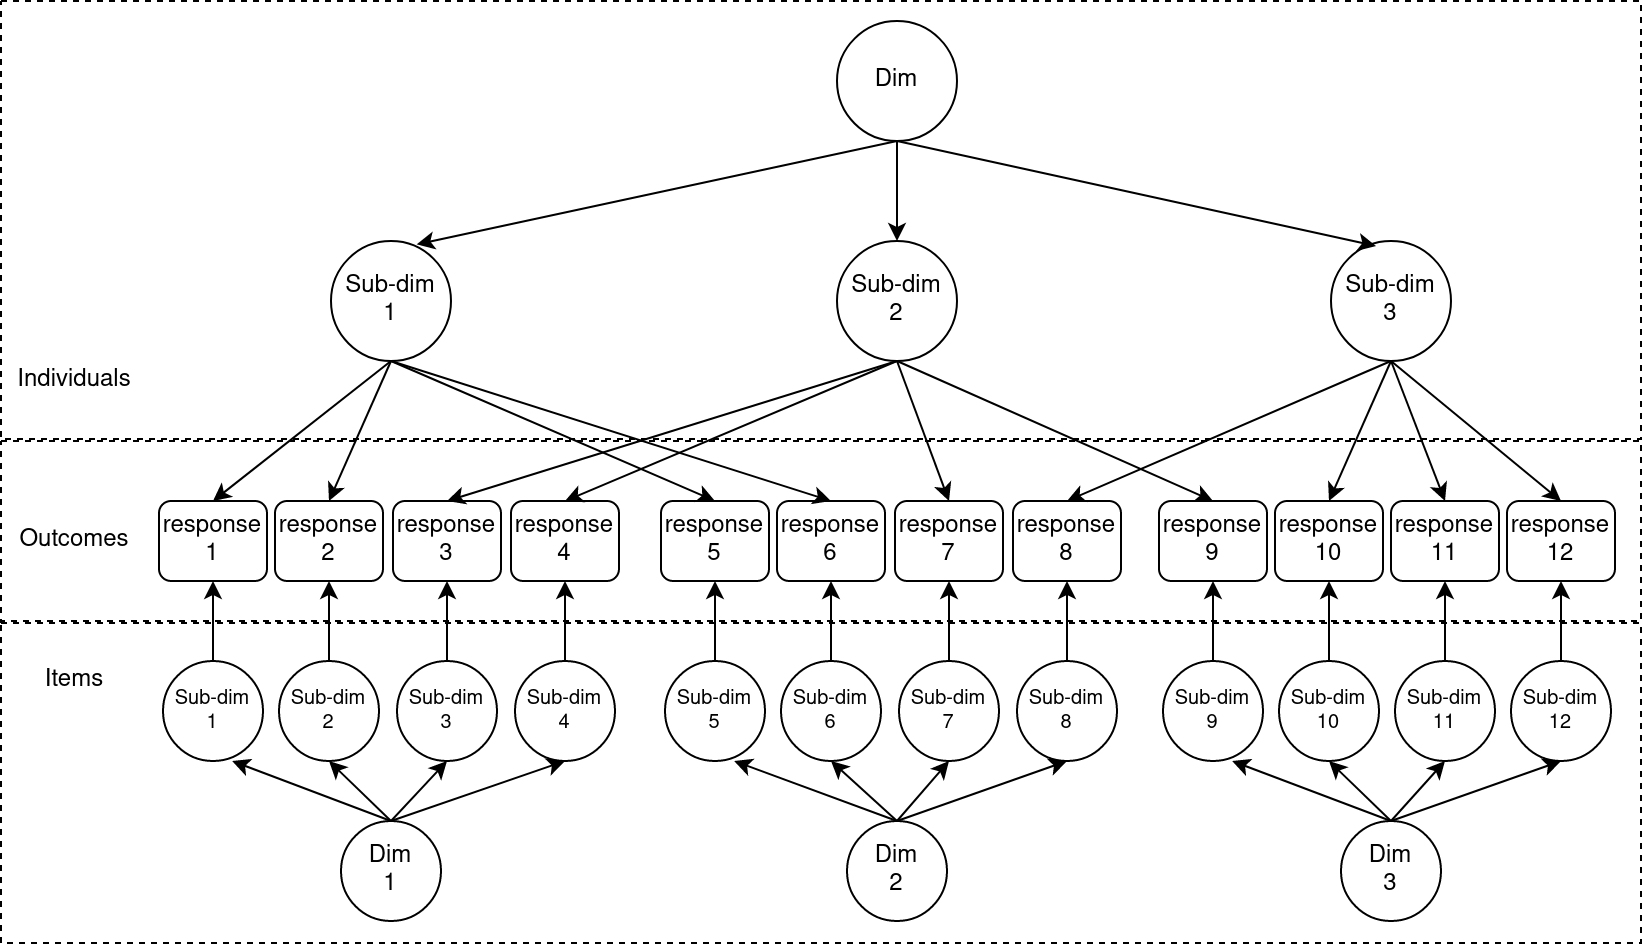
\includegraphics[width=0.9\textwidth]{instrument_design}
		\caption{Path diagram of the dimensional structure for a hierarchical cross-classified IRT model.}
		%\label{fig:design}
	\end{figure}
	%
\end{frame}
%
%---------------------------
\begin{frame}
	%
	\frametitle{Motivating example (cont.)}
	%
	\begin{itemize}
		%
		\item Empty level-1 covariates matrix $\mathbf{X}_{j}$ ($P=0$)
		%
		\item $M=2$ levels at the items block, with $K_{2}=12$ and $K_{3}=3$, i.e. $\pmb{\eta}^{(2)} = [ \eta_{1}^{(2)}, \dots, \eta_{12}^{(2)} ]^{T}$ and $\pmb{\eta}^{(3)} = [ \eta_{1}^{(3)}, \eta_{2}^{(3)}, \eta_{3}^{(3)} ]^{T}$
		%
		\item $L=2$ levels in the individuals block, with $D_{2}=3$ and $D_{3}=1$, i.e. $\pmb{\theta}^{(2)} = [ \theta_{1}^{(2)}, \theta_{2}^{(2)}, \theta_{3}^{(2)} ]^{T}$ and $\pmb{\theta}^{(3)} = \theta_{1}^{(3)}$.
		%
		\item Specific regression relationship among latents $\pmb{\Psi}$, i.e.
		$ \pmb{\alpha}^{(3)} = [ \alpha_{11}^{(3)}, \dots, \alpha_{15}^{(3)}, \alpha_{21}^{(3)}, \dots, \alpha_{25}^{(3)}, \alpha_{31}^{(3)}, \dots, \alpha_{35}^{(3)} ]^{T} $ and  $ \pmb{\lambda}^{(3)} = [ \lambda_{1}^{(3)}, \lambda_{2}^{(3)}, \lambda_{3}^{(3)} ]^{T}$ 
		%
		\item Empty structural covariates $\mathbf{W}$.
		%
	\end{itemize}
	%
\end{frame}
%
%
%%%%%%%%%%%%%%%%%%%%%%%%%%%%%%%%%%%%%%%%%%%%%%%%%%%%%%%%%%%%%%%%%
\section{3. Bayesian estimation}
%%%%%%%%%%%%%%%%%%%%%%%%%%%%%%%%%%%%%%%%%%%%%%%%%%%%%%%%%%%%%%%%%
%
\begin{frame}
	%
	\textbf{3. Bayesian Estimation}
	%
\end{frame}
%
%---------------------------
\begin{frame}
	%
	\frametitle{Bayesian GLLAMM for dichotomous outcomes}
	%
	\begin{enumerate}
		%
		\item \textbf{Posterior distribution.}
		Given that $\mathbf{Y}$ is the observed data and $\pmb{\Omega} = \{ \pmb{\beta}, \pmb{\Lambda}, \pmb{\Theta}, \pmb{\Psi}, \pmb{\Gamma} \}$ the parameters:
		%
		\begin{equation} \label{eq:posterior1}
			\begin{split}
				P(\pmb{\Omega} \; | \; \mathbf{Y}) &= \frac{ P( \mathbf{Y} \; | \; \pmb{\Omega} ) \; P( \pmb{\Omega} ) }{ \int P( \mathbf{Y} \; | \; \pmb{\Omega} ) \; P( \pmb{\Omega} ) \; d\pmb{\Omega} }
			\end{split}
		\end{equation}
		%
		\item \textbf{Prior distributions.}
		Similar to \citet{Patz_et_al_1999}, we use an independent distributional structure for the joint priors:
		%
		\begin{equation}
			\begin{split}
				P( \pmb{\Omega} ) =& P( \pmb{\beta} ) \; \left[ P( \pmb{\alpha} ) \; P( \pmb{\lambda} ) \right] \; \left[ P( \pmb{\eta} ) \; P( \pmb{\theta} ) \right] \\
			%
				& \left[ P( \pmb{\Psi}_{\eta} ) \; P( \pmb{\Psi}_{\theta} ) \right] \; \left[ P( \pmb{\Gamma}_{\eta} ) \; P( \pmb{\Gamma}_{\theta} ) \right]
			\end{split}
		\end{equation}
		%
	\end{enumerate}
	%
\end{frame}
%
%---------------------------
\begin{frame}
	%
	\frametitle{Bayesian GLLAMM for dichotomous outcomes (cont.)}
	%
	\begin{enumerate}
		\setcounter{enumi}{2}
		%
		\item \textbf{Likelihood.}
		Following \citet{Rabe_et_al_2004a}, the likelihood function is build in a recursive way. 
	\end{enumerate}
	%
	\vspace{0.3cm} \begin{equation} \label{eq:dist}
		\footnotesize
		\begin{split}
			f \left( y_{jkd}=1 \; | \; \mathbf{X}, \mathbf{W}, \pmb{\Omega} \right) &= \pi_{jkd}^{n} (1 - \pi_{jkd})^{1-n}
		\end{split}
	\end{equation}
	%
	\begin{equation} \label{eq:lik1}
		\footnotesize
		f \left( \mathbf{y}=\mathbf{1} \; | \; \mathbf{X}, \mathbf{W}, \pmb{\Omega} \right) = \prod_{j=1}^{J} \prod_{d=1}^{D} \prod_{k=1}^{K} f \left( y_{jkd}=1 \; | \; \mathbf{X}, \mathbf{W}, \pmb{\Omega} \right)
	\end{equation}
	%
	\begin{equation} \label{eq:lik2}
		\footnotesize
		f^{(l)}_{(m)} \left( \mathbf{y}=\mathbf{1} \; | \; \mathbf{X}, \mathbf{W}, \pmb{\Omega} \right) = \int \left[ \prod f^{(l-1)}_{(m-1)} \left( \mathbf{y}=\mathbf{1} \; | \; \mathbf{X}, \mathbf{W}, \pmb{\Omega} \right) \right] \; P( \pmb{\Theta}^{(l)}_{(m)} ) \; d\pmb{\Theta}^{(l)}_{(m)}
	\end{equation}
	%
	%
	\begin{equation} \label{eq:lik3}
		\footnotesize
		\mathcal{L}(\mathbf{X}, \mathbf{W}, \pmb{\Omega}) = \prod_{m=2}^{M+1} \prod_{l=2}^{L+1} f^{(l)}_{(m)} \left( \mathbf{y}=\mathbf{1} \; | \; \mathbf{X}, \mathbf{W}, \pmb{\Omega} \right)
	\end{equation}
	%
	%
	\begin{equation} \label{eq:loglik}
		\footnotesize
		\ell(\mathbf{X}, \mathbf{W}, \pmb{\Omega}) = \log \mathcal{L}(\mathbf{X}, \mathbf{W}, \pmb{\Omega})
	\end{equation}
	%
\end{frame}
%
%---------------------------
\begin{frame}
	%
	\frametitle{Computational implementation}
	%
	\begin{enumerate}
		%\setcounter{enumi}{2}
		%
		\item With Hamiltonian Monte Carlo (HMC) and \texttt{Stan} \cite{Stan2020}.
		%
		\item \textbf{No burn-in and thinning}. However, a warm-up phase is required to ``tune-up" the number of steps (\texttt{leapfrogs}), and the \texttt{step size} \cite{Stan2020}.
		%
		\item We will use a total $3,000$ \textbf{effective iterations}, coming from $3$ chains of $2,000$ iterations each, where $1,000$ of them will be spend on warm-up.
		%
		\item \textbf{Initial starts} sampled from the priors defined in the model.
		%
		\item Prior distributions selected based on \textbf{prior predictive simulations}.
		%
	\end{enumerate}
	%
\end{frame}
%
%---------------------------
\begin{frame}
	%
	\frametitle{To center or not to center}
	%
	Even the most simple hierarchical models present formidable pathologies, that no simple rotation/rescaling of the parameter can be performed to visit the posterior distribution properly \cite{Betancourt_et_al_2013}. \\
	%
	\vspace{0.3cm} Example, the devil's funnel \cite{McElreath_2020}:
	%
	%
	\begin{equation} \label{eq:devil}
		\begin{split}	
			v &\sim N(0, 3) \\
			\theta &\sim N(0, \text{exp}(v))
		\end{split}
	\end{equation}
	%
	Equation (\ref{eq:devil}) describes a centered parametrization (CP)
	%
\end{frame}
%
%---------------------------
\begin{frame}
	%
	\frametitle{To center or not to center (cont.)}
	%
	\begin{figure}[h]
		\centering
		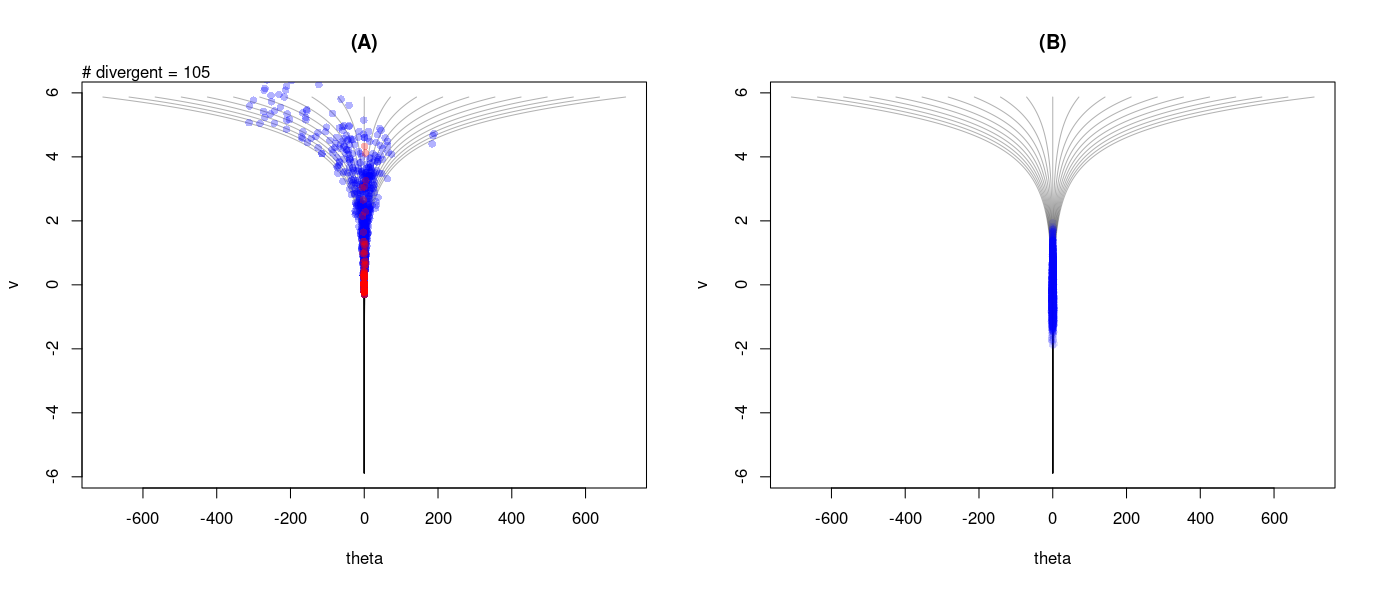
\includegraphics[width=1\linewidth]{1_funnel_CE_simple}
		%
		\caption{Posterior sampling geometry. Centered Parametrization.}
		\label{fig:devil_CE_geom}
	\end{figure}
	%
\end{frame}
%
%---------------------------
\begin{frame}
	%
	\frametitle{To center or not to center (cont.)}
	%
	How can we solve this?:
	%
	\begin{enumerate}
		%\setcounter{enumi}{2}
		%
		\item Adapt HMC warm-up (\texttt{adapt\_delta}$=0.99$).
		%
		\item Use regularizing priors
		%
		\item Use the \textbf{non-centered parametrization}.
		%
	\end{enumerate}
	%
\end{frame}
%
%---------------------------
\begin{frame}
	%
	\frametitle{Non-centered parametrization (NCP)}
	%
	Changing the posterior sampling geometry means to modify equation (\ref{eq:devil}) in the following way:
	%
	\begin{equation} \label{eq:devil_NC}
		\begin{split}	
			v &\sim N(0, 3) \\
			z &\sim N(0, 1) \\
			\theta &= \text{exp}(v) \; z
		\end{split}
	\end{equation}
	%
\end{frame}
%
%---------------------------
\begin{frame}
	%
	\frametitle{Non-centered parametrization (cont.)}
	%
	Changing the posterior sampling geometry means to modify equation (\ref{eq:devil}) in the following way:
	%
	\begin{figure}[h]
		\centering
		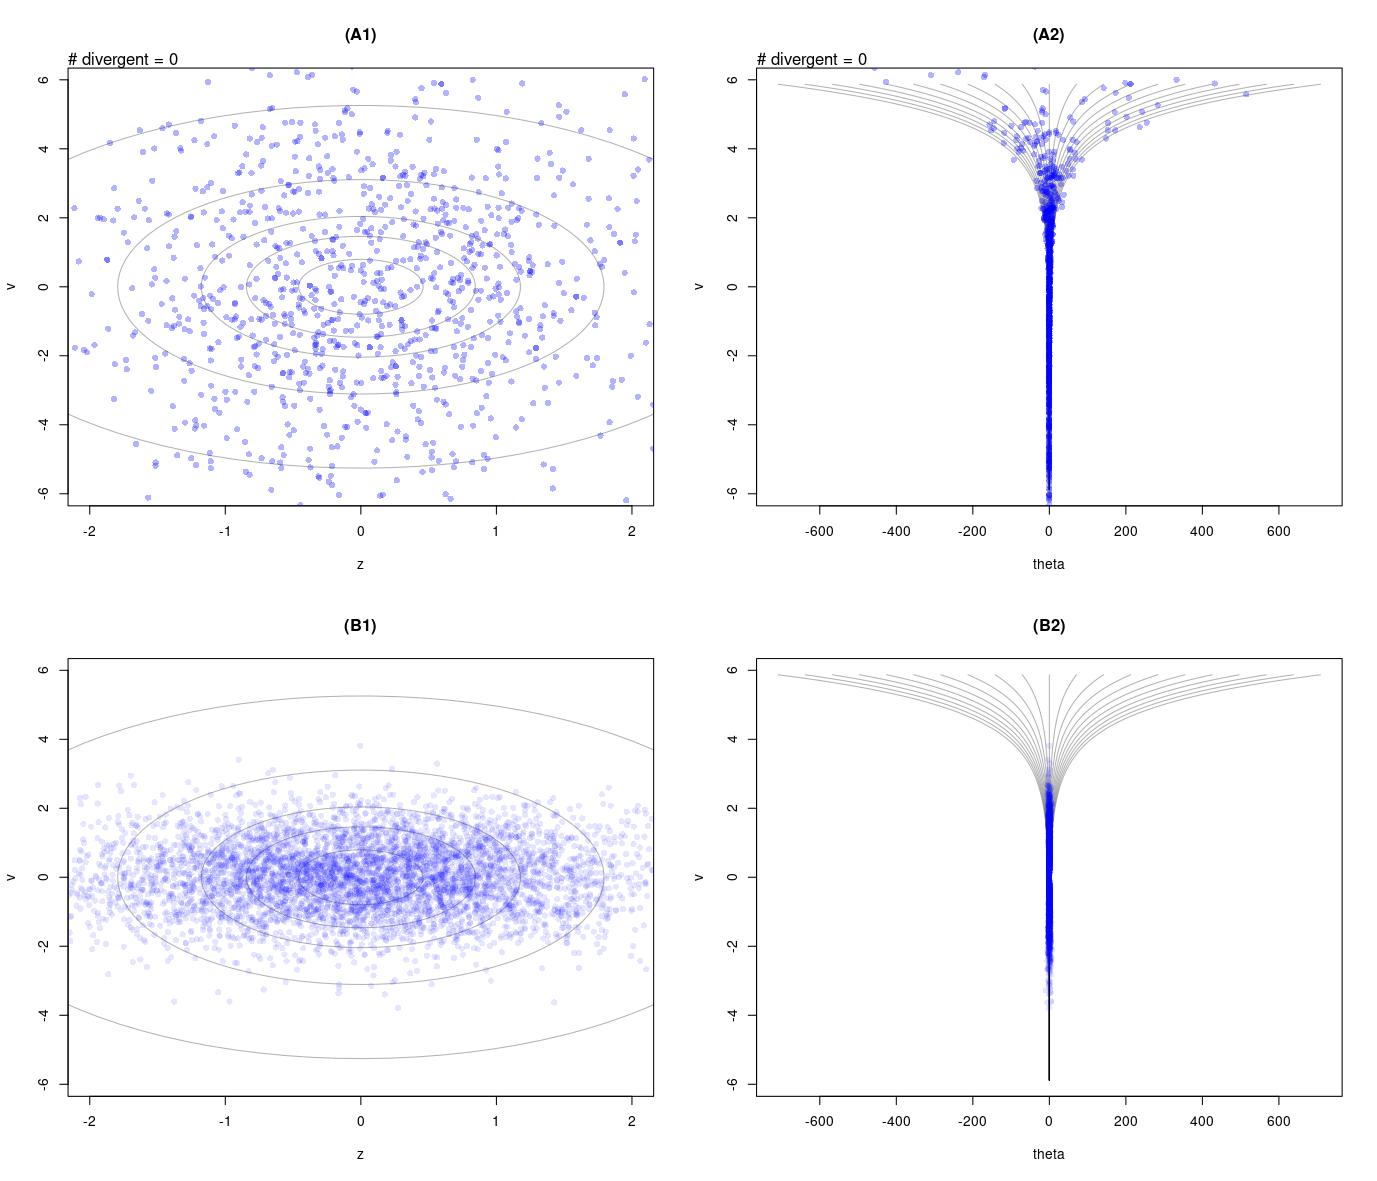
\includegraphics[width=0.55\linewidth]{3_funnel_NC}
		%
		\caption{Posterior sampling geometry. Non-Centered Parametrization.}
		\label{fig:devil_NC_geom}
	\end{figure}
	%
\end{frame}
%
%
%%%%%%%%%%%%%%%%%%%%%%%%%%%%%%%%%%%%%%%%%%%%%%%%%%%%%%%%%%%%%%%%%
\section{4. Simulation study}
%%%%%%%%%%%%%%%%%%%%%%%%%%%%%%%%%%%%%%%%%%%%%%%%%%%%%%%%%%%%%%%%%
%
\begin{frame}
	%
	\textbf{4. Simulation studies}
	%
\end{frame}
%
%---------------------------
\begin{frame}
	%
	\frametitle{Objectives}
	%
	Designed to assess three attributes of the bayesian implementation of the GLLAMM for dichotomous outcomes:
	%
	\begin{enumerate}
		%
		\item \textbf{Performance.} In terms of achieving ergodicity, under the CP and NCP, 
		%
		\item \textbf{Recovery capacity.} Capacity to recover the parameters of interest, especially the structural regression parameters.
		%
		\item \textbf{Retrodictive accuracy.} Capacity to retrodict the data of interest, according to a set of aggregating dimensions.
		%
	\end{enumerate} 
	%
\end{frame}
%
%---------------------------
\begin{frame}
	%
	\frametitle{Evaluation criteria}
	%
	\begin{enumerate}
		%
		\item \textbf{Performance.} Trace, trank and ACF plots with support of \texttt{Rhat} and \texttt{n\_eff} statistics developed by \citet{Gelman_et_al_2014} (pp. $284-287$).
		%
		\item \textbf{Recovery capacity.} we used the between replica root mean squared error ($\text{RMSE}_{B}$).
		%
		\item \textbf{Retrodictive accuracy.} we used the average within $\overline{\text{RMSE}}_{W}$ and between prediction root mean squared error $\text{RMSE}_{B}$, of the responses' predictive proportion $\hat{p}$, versus the observed proportion $p$.
		%
	\end{enumerate} 
	%
\end{frame}
%
%---------------------------
\begin{frame}
	%
	\frametitle{Results \\
		(Performance)}
	%
	\begin{enumerate}
		%
		\item \textbf{Performance.} In terms of achieving ergodicity, under the CP and NCP, 
		%
		\item \textbf{Recovery capacity.} Capacity to recover the parameters of interest, especially the structural regression parameters.
		%
		\item \textbf{Retrodictive accuracy.} Capacity to retrodict the data of interest, according to a set of aggregating dimensions.
		%
	\end{enumerate} 
	%
\end{frame}
%
%---------------------------
\begin{frame}
	%
	\frametitle{Results \\
		(Recovery capacity)}
	%
	\begin{enumerate}
		%
		\item \textbf{Performance.} In terms of achieving ergodicity, under the CP and NCP, 
		%
		\item \textbf{Recovery capacity.} Capacity to recover the parameters of interest, especially the structural regression parameters.
		%
		\item \textbf{Retrodictive accuracy.} Capacity to retrodict the data of interest, according to a set of aggregating dimensions.
		%
	\end{enumerate} 
	%
\end{frame}
%
%---------------------------
\begin{frame}
	%
	\frametitle{Results \\
		(Retrodictive accuracy)}
	%
	\begin{enumerate}
		%
		\item \textbf{Performance.} In terms of achieving ergodicity, under the CP and NCP, 
		%
		\item \textbf{Recovery capacity.} Capacity to recover the parameters of interest, especially the structural regression parameters.
		%
		\item \textbf{Retrodictive accuracy.} Capacity to retrodict the data of interest, according to a set of aggregating dimensions.
		%
	\end{enumerate} 
	%
\end{frame}
%
%
%%%%%%%%%%%%%%%%%%%%%%%%%%%%%%%%%%%%%%%%%%%%%%%%%%%%%%%%%%%%%%%%%
\section{5. Application}
%%%%%%%%%%%%%%%%%%%%%%%%%%%%%%%%%%%%%%%%%%%%%%%%%%%%%%%%%%%%%%%%%
%
\begin{frame}
	%
	\textbf{5. Application}
	%
\end{frame}
%
%---------------------------
\begin{frame}
	%
	\frametitle{Specific goals}
	%
	The research have two main goals:
	%
	\begin{itemize}
		\item to describe the method, estimation procedures, and advantages of the GLLAMM framework, and 
		%
		\item to tests the policy implications of the method and its results, in a data composed of large repeated teacher's standardized educational assessments from Peru. 
		%
	\end{itemize}
	%
\end{frame}
%
%
%%%%%%%%%%%%%%%%%%%%%%%%%%%%%%%%%%%%%%%%%%%%%%%%%%%%%%%%%%%%%%%%%
\section{6. Conclusions}
%%%%%%%%%%%%%%%%%%%%%%%%%%%%%%%%%%%%%%%%%%%%%%%%%%%%%%%%%%%%%%%%%
%
\begin{frame}
	%
	\textbf{6. Conclusions and further development}
	%
\end{frame}
%
%---------------------------
\begin{frame}
	%
	\frametitle{Specific goals}
	%
	The research have two main goals:
	%
	\begin{itemize}
		\item to describe the method, estimation procedures, and advantages of the GLLAMM framework, and 
		%
		\item to tests the policy implications of the method and its results, in a data composed of large repeated teacher's standardized educational assessments from Peru. 
		%
	\end{itemize}
	%
\end{frame}
%
%
%%%%%%%%%%%%%%%%%%%%%%%%%%%%%%%%%%%%%%%%%%%%%%%%%%%%%%%%%%%%%%%%%
\section*{Appendix}
%%%%%%%%%%%%%%%%%%%%%%%%%%%%%%%%%%%%%%%%%%%%%%%%%%%%%%%%%%%%%%%%%
%
\begin{frame}
	%
	\textbf{Appendix}
	%
\end{frame}
%
%---------------------------
\begin{frame}
	%
	\frametitle{Cluster effects}
	%
	Individual clustering involves the addition of more random effects to the linear predictor defined in equation (\ref{eq:linear_predictor1}):
	%
	\begin{equation} \label{eq:linear_predictor4}
		\begin{split}
			v_{jkdc} &= v_{jkd} + \sum_{c=1}^{C} \delta_{c}  \\
			%
			&= v_{jkd} + \pmb{\delta} \mathbf{Z}_{j}
		\end{split}
	\end{equation}
	%
\end{frame}
%
%---------------------------
\begin{frame}
	%
	\frametitle{Example (restrictions for IRT)}
	%
	we could set the restriction $\pmb{\alpha}^{(2)} = -\pmb{\lambda}^{(2)}$ where $\pmb{\lambda}^{(2)} > \mathbf{0}$. In that case we get a multidimensional generalization of the linear predictor observed in the archetypical Rasch \cite{Rasch_1980}, or 2PL \cite{Lord_et_al_2008} models, i.e. $ \lambda^{(2)}_{d} (\theta^{(2)}_{jd} - \eta^{(2)}_{k} )$ \\
	%
	\vspace{0.3cm} In addition, $\pmb{\alpha}^{(3)} = [ \alpha_{11}^{(3)}, \dots, \alpha_{15}^{(3)}, \alpha_{21}^{(3)}, \dots, \alpha_{25}^{(3)}, , \alpha_{31}^{(3)}, \dots, \alpha_{35}^{(3)} ]^{T}$ $= [1,\dots,1]^{T}$, indicating texts difficulties explain directly the items difficulties at the lower level.
	%
\end{frame}
%
%---------------------------
\begin{frame}
	%
	\frametitle{Example (restrictions for IRT)}
	Moreover, notice that because in the IRT framework $\pmb{\eta}$ and $\pmb{\theta}$ should be orthogonal to each other by design, we can further decompose equation (\ref{eq:structural_model1}) in the following form:
	%
	\begin{equation} \label{eq:structural_model2}
		\begin{split}
			\pmb{\eta} = \underset{(K \times K)}{\pmb{\Psi}_{\eta}} \underset{(K \times 1)}{\pmb{\eta}} + \underset{(K \times Q)}{\pmb{\Gamma}_{\eta}} \underset{(Q \times 1)}{\mathbf{W}_{\eta}} + \underset{(K \times 1)}{\pmb{\zeta}_{\eta}}
		\end{split}
	\end{equation}
	%
	\begin{equation} \label{eq:structural_model3}
		\begin{split}
			\pmb{\theta} = \underset{(D \times S)}{\pmb{\Psi}_{\theta}} \underset{(D \times 1)}{\pmb{\theta}} + \underset{(D \times Q)}{\pmb{\Gamma}_{\theta}} \underset{(Q \times 1)}{\mathbf{W}_{\theta}} + \underset{(D \times 1)}{\pmb{\zeta}_{\theta}}
		\end{split}
	\end{equation}
	%
\end{frame}
%---------------------------
\begin{frame}
	%
	\frametitle{Model Assumptions}
	Following \citet{Skrondal_et_al_2004a}, the framework has two main assumptions: 
	%
	\begin{enumerate}
		%\setcounter{enumi}{2}
		\item[\textbf{(M1)}] \textbf{Complete latent space.}\citep{Hambleton_et_al_1991b} In the GLLAMM representation, the space is complete if we consider all latent variables $\pmb{\Theta}$ at levels $l > 1$ and $m > 1$.
		%
		\item[\textbf{(M2)}] \textbf{Local Independence.} It assumes independence conditional on all the latent dimensions and covariates, at different hierarchical levels; effectively modeling all the observed dependencies.
		%
	\end{enumerate}
	%
\end{frame}
%
%---------------------------
\begin{frame}
	%
	\frametitle{Model Assumptions (cont.)}
	\textbf{Local Independence} is defined as follows:
	%
	\begin{equation} \label{eq:independence}
		\footnotesize
		f \left( \mathbf{y} = \mathbf{1} \; | \; \mathbf{X}, \mathbf{W}, \pmb{\Omega} \right) = \prod_{j=1}^{J} \prod_{d=1}^{D} \prod_{k=1}^{K} f \left( y_{jkd}=1 \; | \; \mathbf{X}, \mathbf{W}, \pmb{\Omega} \right)
	\end{equation}
	%
\end{frame}
%
%---------------------------
\begin{frame}
	%
	\frametitle{Model Assumptions (cont.)}
	but comes from:
	%
	\begin{enumerate}
		%
		\item \textbf{Local item independence,}
		%
		\begin{equation}
			\footnotesize
			f \left( y_{j..}=1 \; | \; \mathbf{X}, \mathbf{W}, \pmb{\Omega} \right) = \prod_{d=1}^{D} \prod_{k=1}^{K} f \left( y_{jkd}=1 \; | \; \mathbf{X}, \mathbf{W}, \pmb{\Omega} \right)
		\end{equation}
		%
		\item \textbf{Local individual independence,}
		%
		\begin{equation}
			\footnotesize
			f \left( y_{.kd}=1 \; | \; \mathbf{X}, \mathbf{W}, \pmb{\Omega} \right) = \prod_{j=1}^{J} f \left( y_{jkd}=1 \; | \; \mathbf{X}, \mathbf{W}, \pmb{\Omega} \right)
		\end{equation}
		%
	\end{enumerate}
	%
\end{frame}
%
%---------------------------
\begin{frame}
	%
	\frametitle{Why bayesian?}
	%
	\begin{itemize}
		\item It is built on a simulation-based estimation method, therefore, it can handle all kinds of priors and data-generating processes \cite{Fox_2010}.
		%
		\item While the likelihood for the data and priors for the parameters are used to define the posterior sampling distributions, they can also be used in a generative way \cite{McElreath_2020}. 
		%
		\item Because the procedure integrates prior knowledge about the parameters, it can produce results even in scenarios where the Maximum Likelihood methods (ML) have issues of non-convergence or improper estimation \cite{Skrondal_et_al_2004a, Fox_2010, McElreath_2020}
		%
	\end{itemize}
	%
\end{frame}
%
%---------------------------
\begin{frame}
	%
	\frametitle{There is nothing wrong?}
	%
	\begin{itemize}
		\item It exposes the user to somewhat-arbitrary decisions about the running of the chains, in order to ensure a proper performance (\textbf{solution:} Hamiltonian Monte Carlo (HMC) \cite{Betancourt_et_al_2013} ).
		%
		\item The user can include all type of information through the priors distributions, making their elicitation convenient for manipulation (\textbf{solution:} prior predictive simulations and/or sensitivity analysis).
		%
		\item Visual evaluation of performance, making it hard to assess if a proper posterior investigation have been made \cite{Gelman_et_al_1996a}
		(\textbf{solution:} help of \texttt{Rhat}, \texttt{n\_eff}, and change of posterior sampling geometry).
		%
	\end{itemize}
	%
\end{frame}
%
%---------------------------
\begin{frame}
	%
	\frametitle{There is nothing wrong? (cont.)}
	%
	\begin{itemize}
		\item The procedure makes it hard to discover parameters' lack of identification \cite{Skrondal_et_al_2004a} (\textbf{solution:} regularizing priors ).
		%
		\item Oftentimes the posterior sampling geometry of the model makes it hard to find proper solutions for the parameter space \cite{Betancourt_et_al_2013} (\textbf{solution:} change the posterior sampling geometry).
		%
		\item The greater the complexity of the model, the harder it is to communicate/share and takes more time
		(\textbf{solution:} No solution, but it is a small ``price" to pay).
		%
	\end{itemize}
	%
\end{frame}
%
%---------------------------
\begin{frame}
	%
	\frametitle{There is nothing wrong? (cont.)}
	%
	\begin{itemize}
		\item The procedure makes it hard to discover parameters' lack of identification \cite{Skrondal_et_al_2004a} (\textbf{solution:} regularizing priors ).
		%
		\item Oftentimes the posterior sampling geometry of the model makes it hard to find proper solutions for the parameter space \cite{Betancourt_et_al_2013} (\textbf{solution:} change the posterior sampling geometry).
		%
		\item The greater the complexity of the model, the harder it is to communicate/share and takes more time
		(\textbf{solution:} No solution, but it is a small ``price" to pay).
		%
	\end{itemize}
	%
\end{frame}
%
%---------------------------
\begin{frame}
	%
	\frametitle{Prior elicitation}
	%
	Un-informative priors are not the solution:
	%
	\begin{enumerate}
		%\setcounter{enumi}{2}
		%
		\item Uninformative / weakly-informative latent prior:
		%
		\begin{equation*} \label{eq:prior_el1}
			\footnotesize
			\begin{split}	
				\theta \sim N(0, 100) \quad & \quad \theta \sim N(0, 1) \\
				\text{logit}(p) = \theta \quad & \quad \text{logit}(p) = \theta
			\end{split}
		\end{equation*}
		%
		\item Uninformative / weakly-informative hierarchical latent prior:
		%
		\begin{equation*} \label{eq:prior_el2}
			\footnotesize
			\begin{split}
				v \sim \log N(0, 3) \quad & \quad v \sim \log N(0, 0.5) \\	
				\theta \sim N(0, v) \quad & \quad \theta \sim N(0, v) \\
				\text{logit}(p) = \theta \quad & \quad \text{logit}(p) = \theta
			\end{split}
		\end{equation*}
		%
	\end{enumerate}
	%
\end{frame}
%
%---------------------------
\begin{frame}
	%
	\frametitle{Prior elicitation (cont.)}
	%
	Un-informative priors are not the solution:
	%
	%
	\begin{figure}[!h]
		\centering
		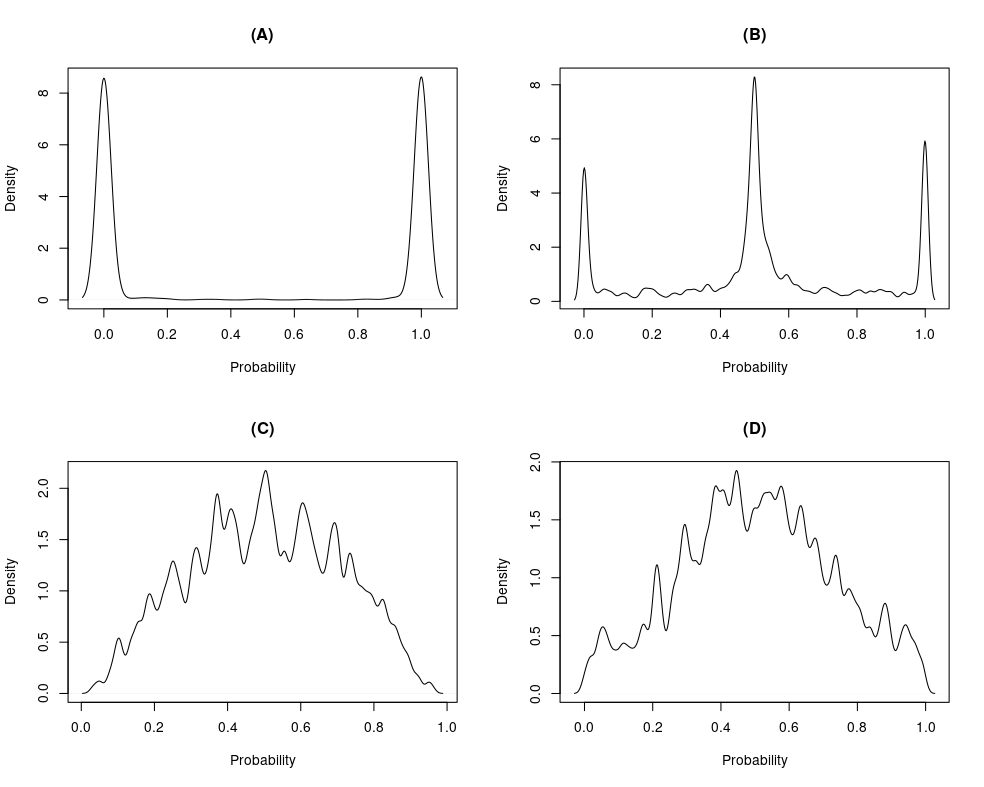
\includegraphics[width=1\textwidth]{prior_elicitation}
		\caption{Prior predictive simulation. Examples of uninformative and mildly informative priors.}
		\label{fig:prior_elicitation}
	\end{figure}
	%
\end{frame}
%
%---------------------------
\begin{frame}
	%
	\frametitle{The benefits of using regularizing priors}
	%
	Consider the use of a regularizing prior on equation (\ref{eq:devil}): 
	%
	\begin{equation} \label{eq:devil_prior}
		\begin{split}	
			v &\sim N(0, 1) \\
			\theta &\sim N(0, \text{exp}(v))
		\end{split}
	\end{equation}
	%
	\begin{figure}[!h]
		\centering
		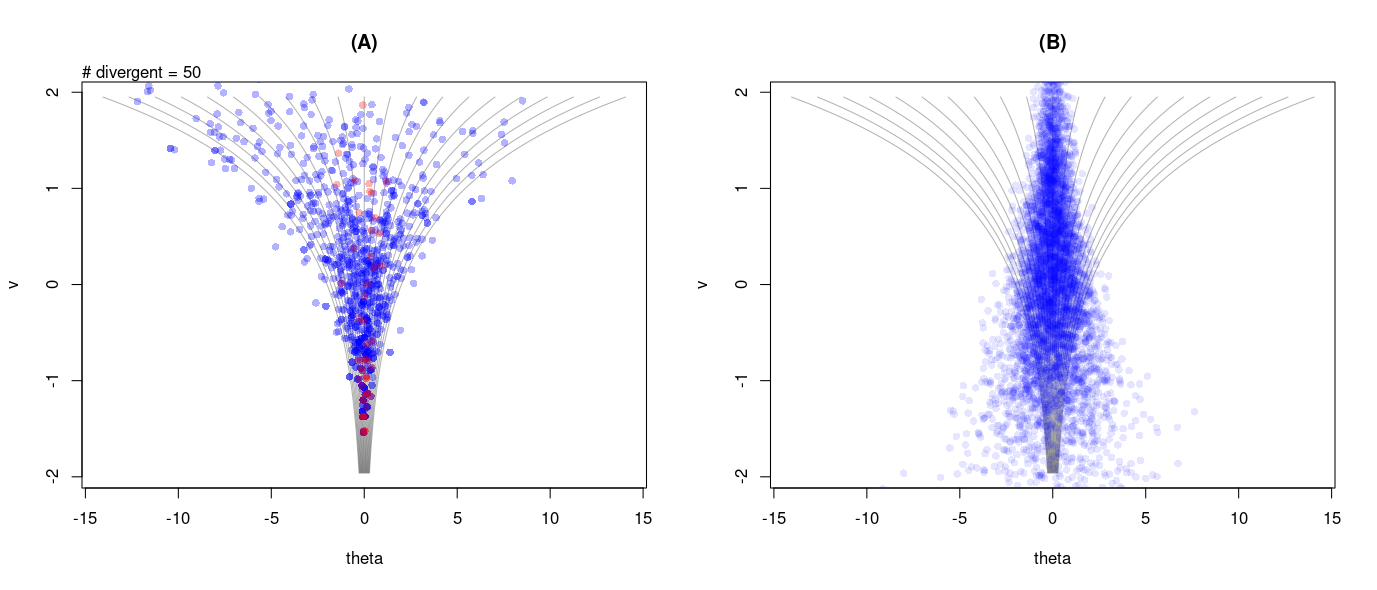
\includegraphics[width=0.8\linewidth]{2_funnel_CE_priors}
		\caption{Posterior sampling geometry. Centered Parametrization with mildly informative priors.}
		\label{fig:devil_prior_geom}
	\end{figure}
	%
\end{frame}
%
%---------------------------
\begin{frame}
	%
	\frametitle{Simulation study design}
	%
	A $3 \times 2 \times 2$ fractional factorial design:
	%
	\begin{itemize}
		\item Three different samples sizes to generate the data under analysis: $500$, $250$, and $100$.
		%
		\item Two parametrization of the models: CP and NCP.
		%
		\item Two models of interest: the first- and second-order latent variable model.
		%
	\end{itemize}
	%
	Ten ($10$) data sets were generated for each study condition. Each data set resembled responses to $25$ binary scored items, conforming to the SOLV model defined in figure \ref{fig:SOLV_model}. The model was motivated by the hypothesized structure of the reading comprehension sub-test, from the Peruvian public teaching career national assessment
	%
\end{frame}
%
%---------------------------
\begin{frame}
	%
	\frametitle{Simulation study design (cont.)}
	%
	\begin{figure}[h]
		\centering
		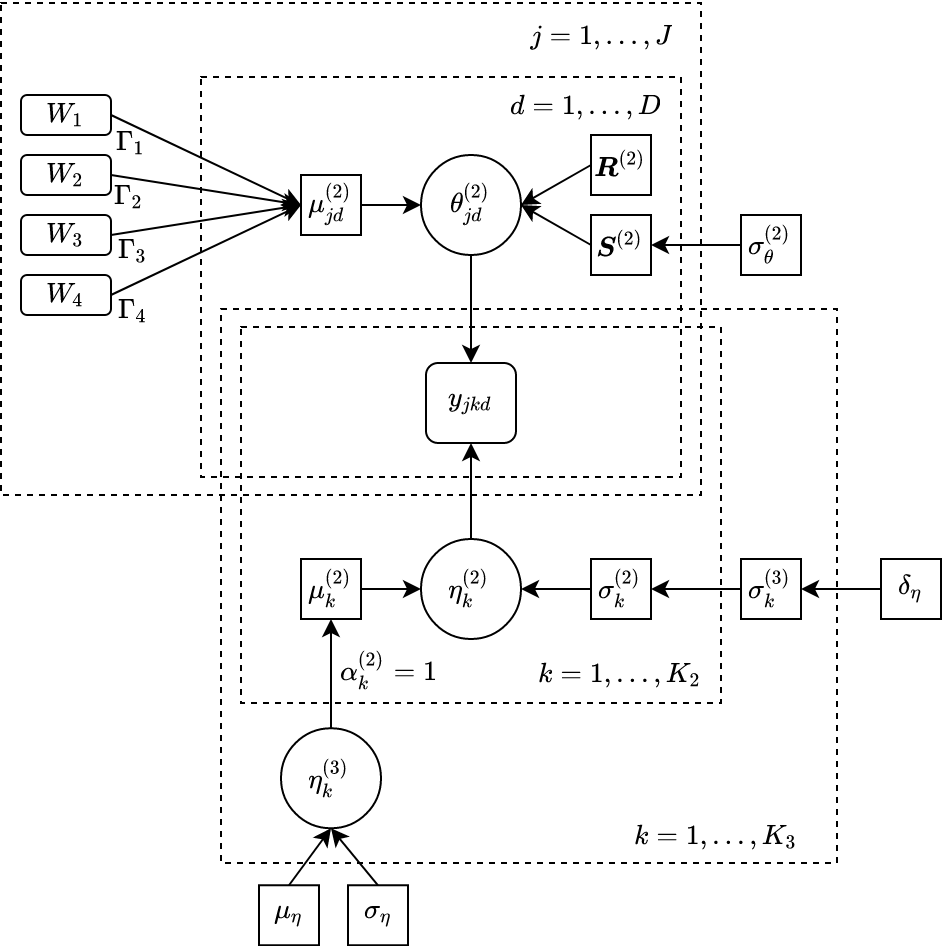
\includegraphics[width=0.5\linewidth]{4_FOLV_dag}
		%
		\caption{Directed Acyclig Graph (DAG). First-order latent variable model (SOLV).}
		\label{fig:FOLV_model}
	\end{figure}
	%
\end{frame}
%
%---------------------------
\begin{frame}
	%
	\frametitle{Simulation study design (cont.)}
	%
	\begin{figure}[h]
		\centering
		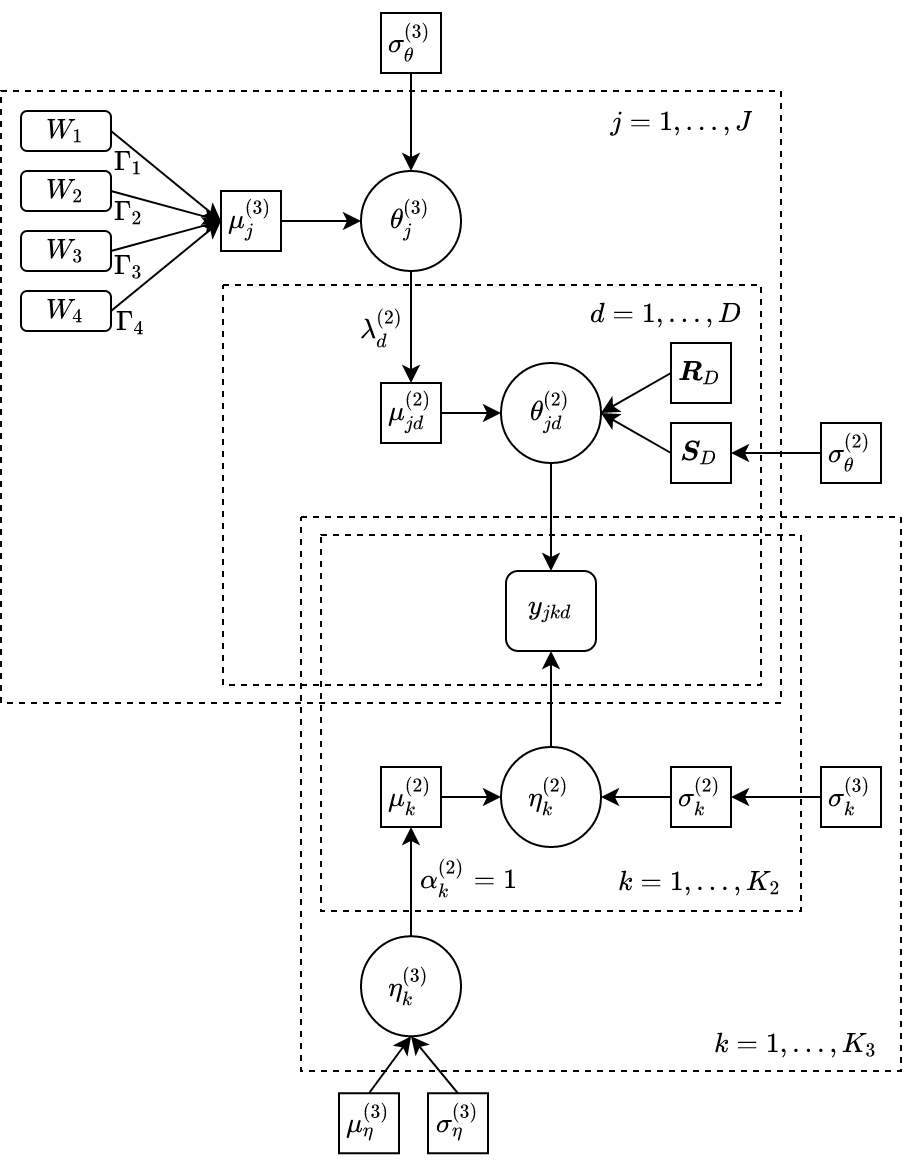
\includegraphics[width=0.50\linewidth]{4_SOLV_dag}
		%
		\caption{Directed Acyclig Graph (DAG). Second-order latent variable model (SOLV).}
		\label{fig:SOLV_model}
	\end{figure}
	%
\end{frame}
%
%---------------------------
\begin{frame}
	%
	\frametitle{Likelihood, priors and hyper-priors
		(centered parametrization)}
	%
	\begin{align}
		%
		y_{jkd} &\sim \text{Bernoulli}( \pi_{jkd} ) \\
		%
		\text{logit}( \pi_{jkd} ) &= v_{jkd} \\
		%
		v_{jkd} &= \theta^{(2)}_{jd} - \eta^{(2)}_{k}
		%
	\end{align}
	%
	\begin{align}
		%
		\boldsymbol{\theta}^{(2)}_{j} &= \left[ \theta_{j1}^{(2)}, \theta_{j2}^{(2)}, \theta_{j3}^{(2)} \right] \\
		%
		\boldsymbol{\theta}^{(2)}_{j} &\sim \text{MVNormal} \left( \boldsymbol{\mu}^{(2)}_{j}, \boldsymbol{\Sigma}^{(2)} \right) \label{eq:theta_sub}
		%
	\end{align}
	%
	%
	\begin{align} \label{eq:sigma_factoring}
		%
		\boldsymbol{\Sigma}^{(2)} &= \boldsymbol{S}^{(2)} \cdot \boldsymbol{R}^{(2)} \cdot \boldsymbol{S}^{(2)} \\
		%
		\boldsymbol{S}^{(2)} &= \pmb{\sigma}^{(2)}_{\theta} \mathbf{I}
		%
	\end{align}
	%
\end{frame}
%
%---------------------------
\begin{frame}
	%
	\frametitle{Likelihood, priors and hyper-priors
		(centered parametrization, cont.)}
	%
	For the FOLV model:
	%
	\begin{align}
		%
		\boldsymbol{\mu}^{(2)}_{j} &= \left[ \mu^{(2)}_{j1}, \; \mu^{(2)}_{j2}, \mu^{(2)}_{j3} \right] \label{eq:mu_FOLV} \\
		%
		\mu^{(2)}_{jd} &= \Gamma_{0} + \Gamma_{1} W_{1j} + \Gamma_{2} (W_{2j} - W_{2\text{min}}) + \Gamma_{3} W_{3j} + \Gamma_{4} W_{4j}
		%
	\end{align}
	%
\end{frame}
%
%---------------------------
\begin{frame}
	%
	\frametitle{Likelihood, priors and hyper-priors
		(centered parametrization, cont.)}
	%
	For the SOLV model:
	%
	\begin{align}
		%
		\boldsymbol{\mu}^{(2)}_{j} &= \left[ \mu^{(2)}_{j1}, \; \mu^{(2)}_{j2}, \mu^{(2)}_{j3} \right] \\
		%
		\pmb{\lambda}^{(2)} &= \left[ \lambda^{(2)}_{1}, \; \lambda^{(2)}_{2}, \lambda^{(2)}_{3} \right] \\
		%
		\mu^{(2)}_{jd} &= \lambda^{(2)}_{d} \; \theta^{(3)}_{j} 
		%
	\end{align}
	%
	%
	\begin{align}
		%
		\theta^{(3)}_{j} &\sim \text{Normal} \left( \mu^{(3)}_{j}, \sigma^{(3)}_{\theta} \right) \label{eq:theta} \\
		%
		\mu^{(3)}_{j} &=  \Gamma_{0} + \Gamma_{1} W_{1j} + \Gamma_{2} (W_{2j} - W_{2\text{min}}) + \Gamma_{3} W_{3j} + \Gamma_{4} W_{4j} \label{eq:mu_SOLV}
	\end{align}
	%
\end{frame}
%
%---------------------------
\begin{frame}
	%
	\frametitle{Likelihood, priors and hyper-priors
		(centered parametrization, cont.)}
	%
	For the items:
	%
	\begin{align}
		%
		\eta^{(2)}_{k} &\sim \text{Normal} \left( \mu^{(2)}_{k}, \sigma^{(2)}_{k} \right) \label{eq:items} \\
		%
		\mu^{(2)}_{k} &= \pmb{\eta}^{(3)} \mathbf{A} \label{eq:mu_items} \\
		%
		\sigma^{(2)}_{k} &= \pmb{\sigma}^{(3)} \mathbf{A} \label{eq:sigma_items} \\
		%
		\pmb{\eta}^{(3)} &= [ \eta^{(3)}_{1}, \eta^{(3)}_{2}, \eta^{(3)}_{3}, \eta^{(3)}_{4}, \eta^{(3)}_{5} ] \\
		%
		\pmb{\sigma}^{(3)} &= [ \sigma^{(3)}_{1}, \sigma^{(3)}_{2}, \sigma^{(3)}_{3}, \sigma^{(3)}_{4}, \sigma^{(3)}_{5} ]
		%
	\end{align}
	%
	\begin{align}
		%
		\eta^{(3)}_{k} &\sim \text{Normal} \left( \mu_{\eta}, \sigma_{\eta} \right) \\
		%
		\sigma^{(3)}_{k} &\sim \text{Exponential} \left( \delta_{\eta} \right)
		%
	\end{align}
	%
\end{frame}
%
%---------------------------
\begin{frame}
	%
	\frametitle{Likelihood, priors and hyper-priors
		(centered parametrization, cont.)}
	%
	Remaining priors and hyper-priors
	%
	\begin{align}
		\boldsymbol{R}^{(2)} &\sim \text{LkjCorrelation}( 2 ) \\
		\Gamma_{1c} &\sim \text{Normal}( 0, 0.5 ) \\
		\Gamma_{2} &\sim \text{Normal}( 0, 0.5 ) \\
		\Gamma_{3c} &\sim \text{Normal}( 0, 1 ) \\
		\Gamma_{4c} &\sim \text{Normal}( 0, 0.5 ) 
		%
	\end{align}
	%
\end{frame}
%
%---------------------------
\begin{frame}
	%
	\frametitle{Likelihood, priors and hyper-priors
		(Non-centered parametrization)}
	%
	Under the NCP, equation (\ref{eq:items}) was re-defined as follows:
	%
	\begin{align}
		%
		\eta^{(2)}_{k} &= \mu^{(2)}_{k} + \sigma^{(2)}_{k} z^{(2)}_{k} \\
		%
		z^{(2)}_{k} &\sim \text{Normal}(0,1)
		%
	\end{align}
	%
	Equation (\ref{eq:theta_sub}) was re-defined as follows:
	%
	\begin{align}
		%
		\boldsymbol{\theta}^{(2)}_{j} &= \boldsymbol{\mu}^{(2)}_{j} + \boldsymbol{S}^{(2)} \cdot \boldsymbol{L}^{(2)}_{\Sigma} \cdot  (\mathbf{z}_{j} \mathbf{I}) \\
		%
		\mathbf{z}_{j} &= [ z_{j1}, \dots, z_{jd}]^{T} \\
		%
		z_{jd} &\sim \text{Normal}(0,1) \\
		%
		\boldsymbol{L}^{(2)}_{\Sigma} &\sim \text{LKJCorrelationCholesky}(2)
		%
	\end{align}
	%
\end{frame}
%
%---------------------------
\begin{frame}
	%
	\frametitle{Likelihood, priors and hyper-priors
		(Non-centered parametrization, cont.)}
	%
	Finally, equation (\ref{eq:theta}) was re-defined as follows:
	%
	\begin{align}
		%
		\theta^{(3)}_{j} &= \mu^{(3)}_{j} + \sigma^{(3)}_{\theta} z_{j} \\
		%
		z_{j} &\sim \text{Normal}(0,1)
		%
	\end{align}
	%
\end{frame}
%
%---------------------------
\begin{frame}
	%
	\frametitle{Identification}
	%
	We used the unit variance identification scheme (UVI), that is, to set the scale of the higher-order dimension and sub-dimensions to one:
	%
	\begin{itemize}
		\item $\sigma^{(3)}_{\theta} = 1$
		%
		\item $\mathbf{S}^{(2)} = \pmb{\sigma}^{(2)}_{\theta} \mathbf{I}$ with $\pmb{\sigma}^{(2)}_{\theta} = [1, 1, 1]^{T}$
		%
		\item $\mu_{\eta} = 0$, $\sigma_{\eta}=1$, $\delta_{\eta}=2$
	\end{itemize}
	%
	The first two turned the covariance matrix into a correlation, i.e. $\boldsymbol{\Sigma}^{(2)} = \boldsymbol{R}^{(2)}$.
	%
\end{frame}
%
%---------------------------
\begin{frame}
	%
	\frametitle{Prior predictive investigation}
	%
	From two perspectives:
	%
	\begin{itemize}
		\item the IRT perspective
		%
		\item the outcome perspective
	\end{itemize}
	% 
\end{frame}
%
%---------------------------
\begin{frame}
	%
	\frametitle{Prior predictive investigation (cont.)}
	%
	From the IRT perspective:
	%
	\begin{figure}[H]
		\centering
		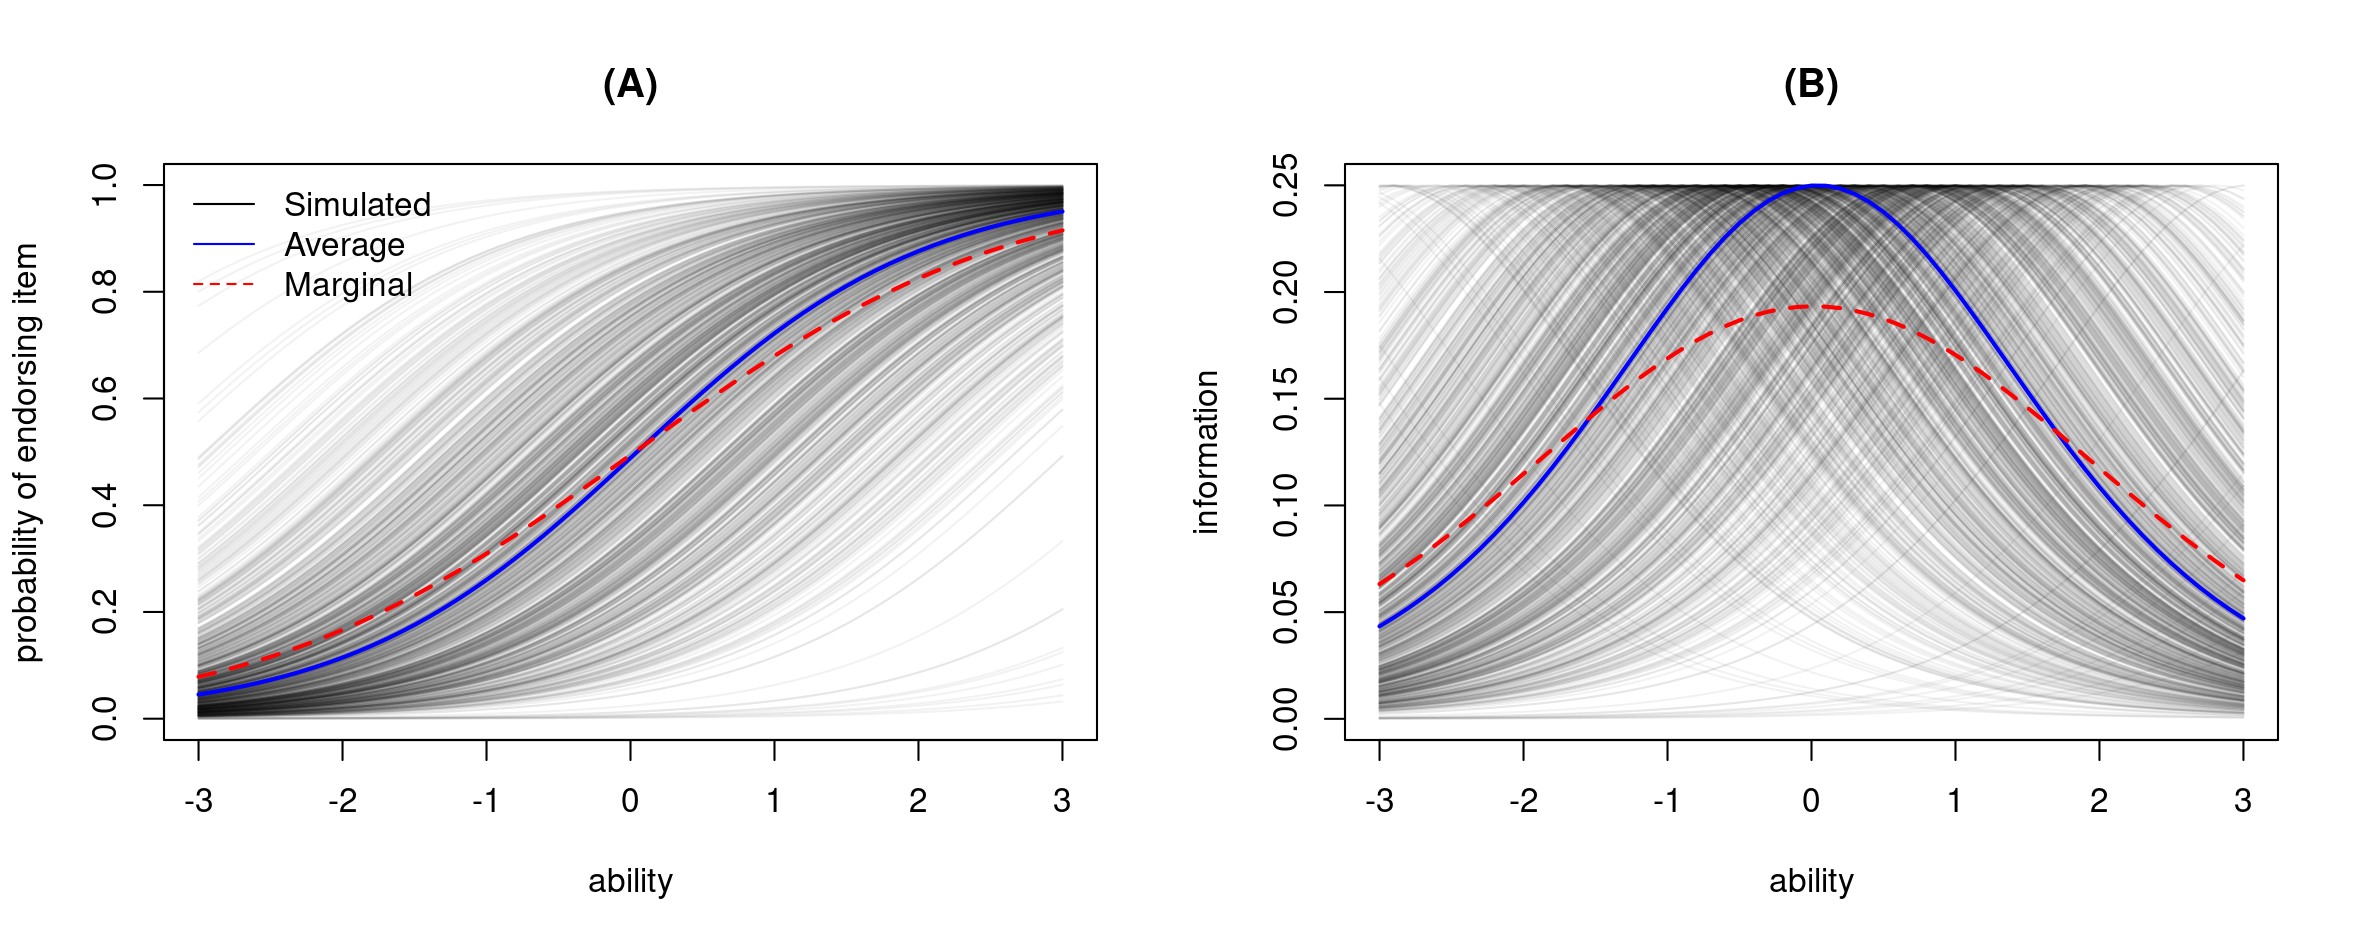
\includegraphics[width=1\linewidth]{FOLV_ICC_prior}
		%
		\caption{First-order latent variable model (FOLV). (A) Item Characteristics Curve, ICC. (B) Item Information Function, IIF.}
		\label{fig:FOLV_ICC_prior}
	\end{figure} 
	%
\end{frame}
%
%---------------------------
\begin{frame}
	%
	\frametitle{Prior predictive investigation (cont.)}
	%
	From the outcome perspective:
	%
	\begin{figure}[h]
		\centering
		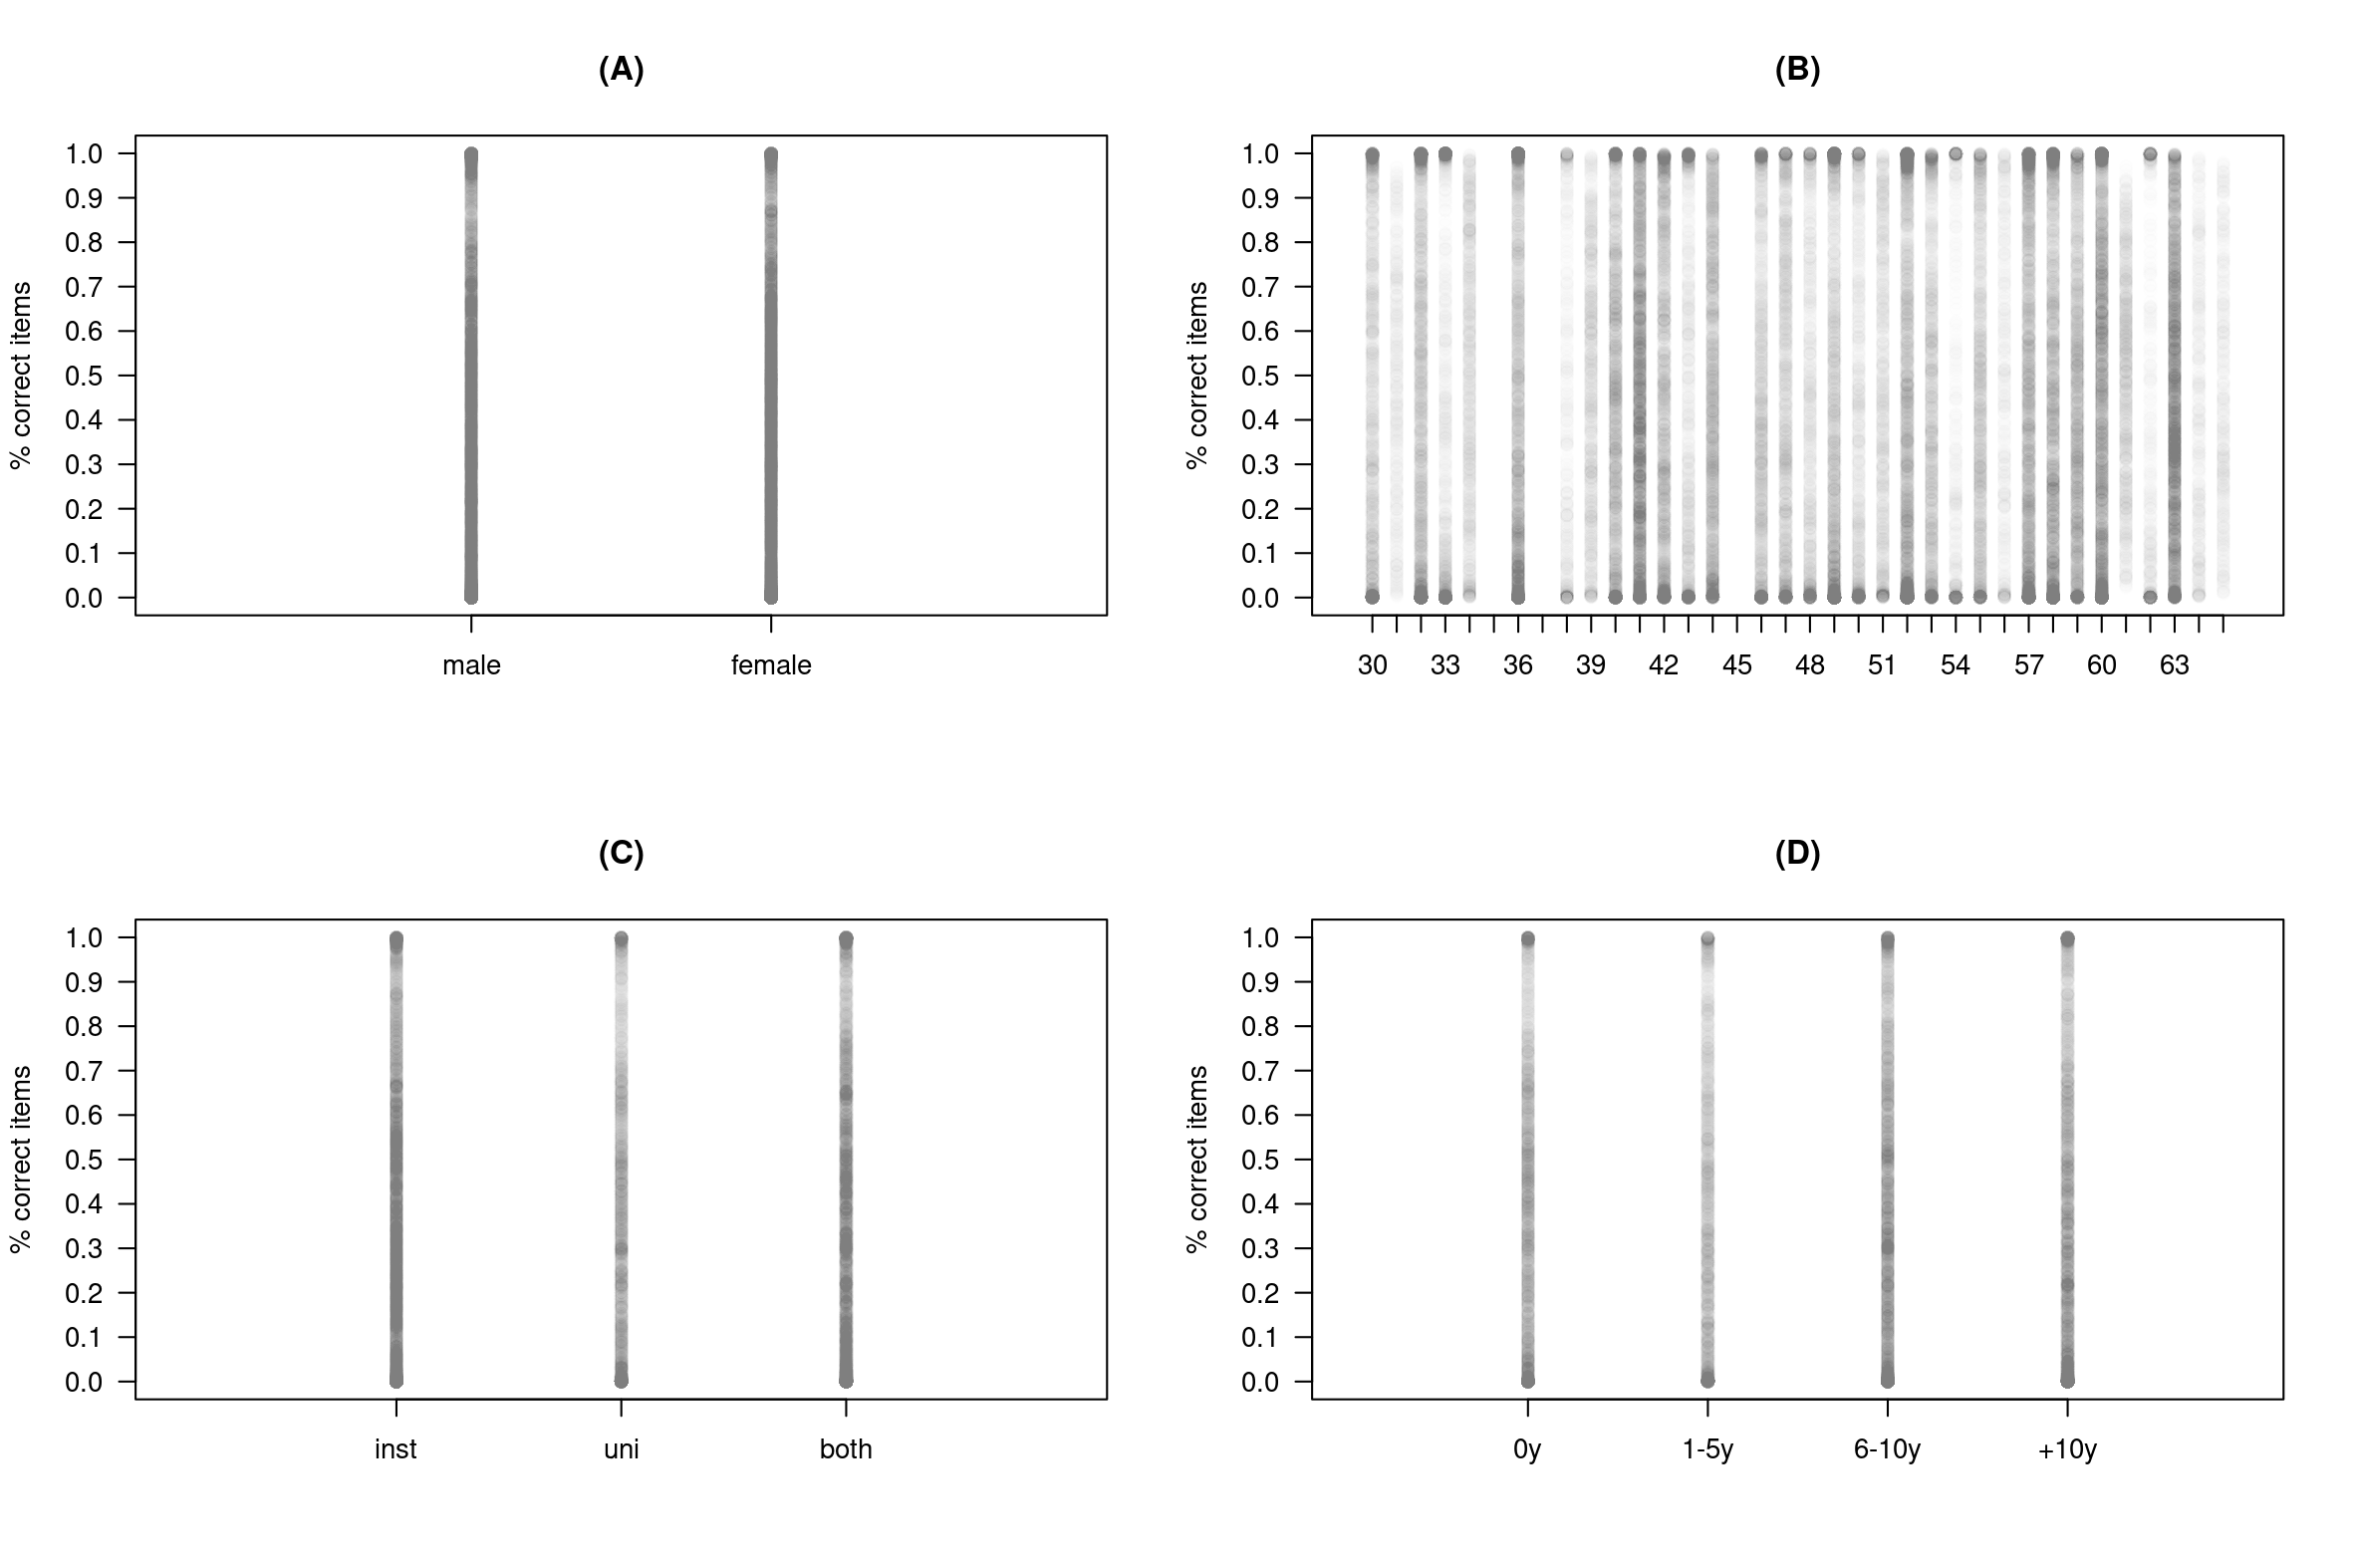
\includegraphics[width=0.65\linewidth]{FOLV_HitRate2}
		%
		\caption{First-order latent variable model (FOLV). Aggregated endorsement rate per simulated covariate: (A) gender, (B) age, (C) education, and (D) experience.}
		\label{fig:FOLV_hitrate2}
	\end{figure}
	% 
\end{frame}
%
%
%%%%%%%%%%%%%%%%%%%%%%%%%%%%%%%%%%%%%%%%%%%%%%%%%%%%%%%%%%%%%%%%%
% Bibliography
%%%%%%%%%%%%%%%%%%%%%%%%%%%%%%%%%%%%%%%%%%%%%%%%%%%%%%%%%%%%%%%%%
%
\begin{frame}[allowframebreaks]
\frametitle{References}
%
%\renewcommand{\harvardand}{y} 	% cambiar "and" por "y" al generar la bibliografia.
\bibliographystyle{dcu}
\bibliography{bibliography}
%
\end{frame}
%
%
\end{document}